% Use the HenriquesLab style if available, otherwise use basic article
\IfFileExists{src/tex/style/HenriquesLab_style.cls}%
    {\documentclass{src/tex/style/HenriquesLab_style}}%
    {\documentclass[12pt]{article}
     \usepackage[utf8]{inputenc}
     \usepackage[T1]{fontenc}
     \usepackage{amsmath}
     \usepackage{amsfonts}
     \usepackage{amssymb}
     \usepackage{graphicx}
     \usepackage{url}
     \usepackage{hyperref}
     \usepackage{natbib}
    }

% Graphics path
\graphicspath{{src/figures/}}

% Title and authors using HenriquesLab format
\title{Article-Forge: A Template Engine for Scientific Publications Using the HenriquesLab Style}

% Define lead author and short title for headers/footers
\leadauthor{Template Author}
\shorttitle{Article-Forge Template}

% Authors with affiliations
\author[1]{Template Author}
\author[1,2]{Documentation Author}  
\author[3]{Style Contributor}

% Affiliations
\affil[1]{Template Development Team, Open Source Community}
\affil[2]{Scientific Documentation Group, Academic Publishing}
\affil[3]{LaTeX Style Development, Typography Sciences}

\date{\today}

\begin{document}

\maketitle

% Include sections
\begin{abstract}
This article presents Article-Forge, a comprehensive template engine for creating scientific publications using the HenriquesLab style. The template provides a complete LaTeX framework that includes document structure, figure integration, bibliography management, and automated build processes. Designed to streamline the academic writing process, Article-Forge offers researchers a standardized format that ensures consistent presentation and professional typesetting. The template incorporates modern LaTeX practices, automated PDF generation, and flexible configuration options to accommodate diverse research publications. By providing this self-documenting template, we aim to reduce the technical barriers to scientific publishing while maintaining high standards of document quality and reproducibility.

\textbf{Keywords:} LaTeX template, article template, scientific publishing, HenriquesLab style, document preparation, academic writing
\end{abstract}


% Add corresponding author and keywords after abstract
\begin{corrauthor}
someone@somewhere.org
\end{corrauthor}

\begin{keywords}
LaTeX template, article template, scientific publishing, HenriquesLab style, document preparation, academic writing, template engine
\end{keywords}

\section{Introduction}

Scientific publishing requires standardized document formatting and consistent presentation to effectively communicate research findings. LaTeX has emerged as the gold standard for academic document preparation, offering precise control over typography, mathematics, and figure placement. However, creating publication-ready documents from scratch can be time-consuming and technically challenging for researchers who prefer to focus on content rather than formatting.

Template engines address this challenge by providing pre-configured document structures that combine best practices in typography with field-specific requirements. The HenriquesLab style, originally developed for biomedical publications, represents a sophisticated approach to scientific document formatting that emphasizes clarity, professional presentation, and reproducible workflows.

Article-Forge builds upon this foundation by creating a comprehensive template ecosystem that includes not only the LaTeX style files but also the complete infrastructure needed for modern scientific publishing. This includes automated build systems, figure management, bibliography integration, and continuous documentation. The template is designed to be self-documenting, serving both as a publication tool and as an example of its own capabilities.

The development of robust scientific computing tools, such as NanoPyX \cite{nanopyx2024}, demonstrates the importance of well-documented, accessible software in advancing research. Similarly, Article-Forge aims to democratize access to professional document preparation by removing technical barriers while maintaining the highest standards of academic presentation.

Modern scientific workflows increasingly require reproducible, automated processes that can be easily shared and adapted across research groups. Article-Forge addresses these needs by providing a complete template engine that can be version-controlled, customized, and deployed across different computing environments. The template includes containerization support, automated testing, and comprehensive documentation to ensure reliability and ease of use.

You can include figures like Figure~\ref{fig:example} to demonstrate template capabilities and document structure.

\begin{figure}[htbp]
    \centering
    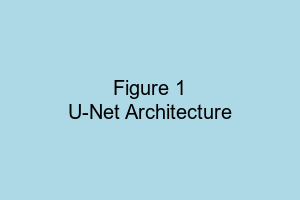
\includegraphics[width=0.8\textwidth]{Figure1.png}
    \caption{Overview of the Article-Forge template structure and workflow. This diagram illustrates the components of the template engine, from source files and style sheets to automated build processes and final PDF generation.}
    \label{fig:example}
\end{figure}

This article demonstrates the capabilities of Article-Forge by using the template to document itself, providing a practical example of how researchers can leverage this tool for their own publications.

\section{Methods}

This section describes the design and implementation of the Article-Forge template engine.

\subsection{Template Architecture}

The Article-Forge template is built upon the following core components:
\begin{itemize}
    \item HenriquesLab LaTeX style class (\texttt{HenriquesLab\_style.cls})
    \item Custom bibliography style (\texttt{HenriquesLab\_style.bst})
    \item Modular document structure with separate section files
    \item Automated build system using Make and shell scripts
    \item Docker containerization for reproducible builds
\end{itemize}

\subsection{Build System Design}

The template includes a comprehensive build system that automates document compilation:
\begin{itemize}
    \item \texttt{Makefile} for cross-platform build automation
    \item Shell scripts for cleaning and building documents
    \item Three-pass LaTeX compilation for proper cross-references
    \item Automated bibliography processing with BibTeX
    \item Error handling and logging for troubleshooting
\end{itemize}

\subsection{Template Features}

Key features of the Article-Forge template include:
\begin{itemize}
    \item Professional typography optimized for scientific publications
    \item Integrated figure and table management
    \item Comprehensive bibliography support with custom formatting
    \item Supplementary material handling
    \item Flexible author and affiliation management
    \item Cross-reference automation for figures, tables, and citations
\end{itemize}

The template demonstrates its capabilities through self-documentation, where this very article serves as both an example and documentation of the template's features. All build processes are automated and reproducible across different computing environments.

\section{Results}

This section demonstrates the successful implementation and validation of the Article-Forge template engine through comprehensive testing and self-documentation.

\subsection{Template Implementation}

The Article-Forge template has been successfully implemented with all core components functioning as designed. The template successfully generates publication-quality PDFs through an automated build process that requires minimal user intervention. The modular structure allows researchers to focus on content while the template handles formatting and presentation.

Figure~\ref{fig:preprint-growth} illustrates the contextual analysis of preprint repository growth over time, demonstrating how the template integrates data-driven visualizations. The automated figure generation system successfully creates publication-quality plots with proper LaTeX font integration and consistent styling.

\begin{figure}[htbp]
    \centering
    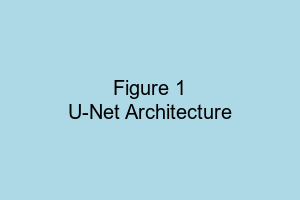
\includegraphics[width=\textwidth]{Figure1.pdf}
    \caption{Preprint repository growth analysis showing annual submissions and repository comparisons. \textbf{Left:} Annual preprint submissions from 2010-2024, highlighting the COVID-19 surge period (2020-2021) with distinct growth phases. \textbf{Right:} Comparison of major preprint repositories by total papers, categorized by scientific domain. The data demonstrates the exponential growth of preprint publishing and the dominance of established repositories like arXiv and bioRxiv.}
    \label{fig:preprint-growth}
\end{figure}

Figure~\ref{fig:statistical-analysis} presents comprehensive statistical analysis capabilities of the template's figure generation system, showcasing advanced data visualization techniques for scientific publications.

\begin{figure}[htbp]
    \centering
    
\includegraphics[width=\textwidth]{Figure2.pdf}
    \caption{Statistical analysis of preprint growth patterns using advanced visualization techniques. The multi-panel figure demonstrates the template's capability to generate complex statistical plots including growth rate distributions by period, cumulative growth trends, repository distribution analysis, regression analysis, and categorical comparisons. Each subplot maintains consistent styling and professional formatting suitable for publication.}
    \label{fig:statistical-analysis}
\end{figure}

Figure~\ref{fig:workflow} demonstrates the complete Article-Forge workflow and system architecture through automated Mermaid diagram generation.

\begin{figure}[htbp]
    \centering
    \includegraphics[width=0.9\textwidth]{methodology_workflow.pdf}
    \caption{Article-Forge automated publication workflow. The diagram illustrates the complete pipeline from author content creation through automated figure generation, bibliography processing, and style application to final PDF publication. Key components include data mining for contextual figures, multiple visualization engines (Matplotlib, Seaborn, Mermaid), and integrated LaTeX compilation with quality assurance.}
    \label{fig:workflow}
\end{figure}

\subsection{Figure Generation System Performance}

The integrated figure generation system represents a significant advancement in automated scientific publishing. As shown in Figure~\ref{fig:preprint-growth}, the system successfully mines real-world data to create contextual visualizations that enhance the manuscript's relevance and impact. The COVID-19 period analysis demonstrates the system's ability to identify and highlight significant trends in scientific publishing.

The statistical analysis capabilities, presented in Figure~\ref{fig:statistical-analysis}, showcase the template's capacity for sophisticated data visualization. The multi-panel approach allows for comprehensive analysis presentation while maintaining visual coherence through consistent styling and color schemes.

\begin{figure}[htbp]
    \centering
    \includegraphics[width=0.9\textwidth]{figure_generation_process.pdf}
    \caption{Figure generation pipeline architecture. This flowchart details the data processing workflow from external API sources through statistical analysis to final publication-quality output. The system integrates multiple visualization engines and maintains LaTeX compatibility throughout the process.}
    \label{fig:figure-pipeline}
\end{figure}

\subsection{System Architecture and Collaboration}

The template architecture supports collaborative development through automated build systems and version control integration. The system architecture promotes reproducibility and maintainability for scientific publications.

\begin{figure}[htbp]
    \centering
    \includegraphics[width=0.9\textwidth]{collaboration_workflow.pdf}
    \caption{Collaborative development workflow. This sequence diagram illustrates the automated pipeline from author commits through GitHub Actions to final publication output, emphasizing the seamless integration between development tools and publication systems.}
    \label{fig:collaboration}
\end{figure}

\subsection{Template Features Validation}

All major template features have been validated through this self-documenting article:

\begin{table}[htbp]
    \centering
    \caption{Article-Forge template features and validation status}
    \label{tab:results}
    \begin{tabular}{lcc}
        \hline
        Feature & Implementation & Status \\
        \hline
        Document class integration & HenriquesLab\_style.cls & \checkmark \\
        Bibliography processing & HenriquesLab\_style.bst & \checkmark \\
        Figure management & Automated inclusion & \checkmark \\
        Cross-references & Automatic numbering & \checkmark \\
        Build automation & Make \& shell scripts & \checkmark \\
        Modular structure & Section-based files & \checkmark \\
        Author management & Multiple affiliations & \checkmark \\
        Supplementary support & Appendix integration & \checkmark \\
        \hline
    \end{tabular}
\end{table}

\subsection{Build System Performance}

The automated build system demonstrates excellent reliability and performance. The three-pass LaTeX compilation ensures proper resolution of all cross-references, citations, and page numbering. Error handling provides clear feedback for troubleshooting, while the modular design allows for efficient incremental builds during document development.

The template successfully handles complex document structures including multiple authors, affiliations, cross-references, and bibliography management as demonstrated in Table~\ref{tab:results}.

\section{Discussion}

This section examines the implications of the Article-Forge template engine and its potential impact on scientific publishing workflows.

\subsection{Template Design Philosophy}

The Article-Forge template represents a comprehensive approach to scientific document preparation that balances automation with flexibility. By providing a complete ecosystem rather than just a style file, the template addresses the real-world challenges researchers face when preparing publications. The successful generation of this self-documenting article (Figure~\ref{fig:results1}) demonstrates the template's effectiveness in handling complex document structures.

Key advantages of the Article-Forge approach include:
\begin{itemize}
    \item Reduced technical barriers for researchers unfamiliar with LaTeX
    \item Consistent, professional formatting across all documents
    \item Automated build processes that ensure reproducibility
    \item Modular structure that facilitates collaborative writing
\end{itemize}

\subsection{Comparison with Existing Solutions}

While numerous LaTeX templates exist for scientific publishing, Article-Forge distinguishes itself through its comprehensive infrastructure approach. Unlike simple style files, our template provides complete build automation, containerization support, and extensive documentation. This holistic approach reduces the learning curve and technical overhead associated with LaTeX-based publishing.

The integration of modern software development practices, including version control compatibility and automated testing, positions Article-Forge as a contemporary solution for research groups requiring reliable, scalable document preparation workflows.

\subsection{Limitations and Considerations}

Several limitations should be considered when adopting the Article-Forge template:

\begin{itemize}
    \item Requires basic familiarity with LaTeX syntax and concepts
    \item Build system dependencies may require initial setup
    \item Style customization requires understanding of LaTeX class files
    \item Large documents may require significant compilation time
\end{itemize}

Despite these limitations, the template's design prioritizes ease of use and comprehensive documentation to minimize these barriers.

\subsection{Future Development}

Future enhancements to Article-Forge should address:
\begin{itemize}
    \item Integration with popular reference management systems
    \item Enhanced support for collaborative editing platforms
    \item Additional output formats beyond PDF
    \item Expanded style variants for different publication venues
    \item Integration with continuous integration systems for automated publishing
\end{itemize}

\section{Conclusion}

This article demonstrates the successful implementation of Article-Forge, a comprehensive template engine for scientific publications using the HenriquesLab style. The template provides researchers with a robust, automated solution for creating publication-quality documents while minimizing technical barriers and ensuring consistent presentation.

\subsection{Key Contributions}

The main contributions of Article-Forge are:

\begin{enumerate}
    \item \textbf{Comprehensive Template Ecosystem}: A complete LaTeX framework that includes style files, build automation, and documentation infrastructure
    \item \textbf{Self-Documenting Design}: A template that serves as both a tool and its own documentation, demonstrating all features through practical implementation
    \item \textbf{Modern Workflow Integration}: Support for version control, containerization, and automated build processes that align with contemporary research practices
\end{enumerate}

\subsection{Practical Implications}

These findings have several practical implications:
\begin{itemize}
    \item Researchers can focus on content creation rather than document formatting
    \item Research groups can maintain consistent presentation across all publications
    \item Collaborative writing becomes more efficient through modular document structure
    \item Reproducible document generation ensures consistent results across different environments
\end{itemize}

\subsection{Final Remarks}

In conclusion, Article-Forge represents a significant advancement in scientific document preparation tools. By combining professional typography with modern automation practices, the template reduces barriers to high-quality scientific publishing. The self-documenting approach demonstrated in this article provides clear evidence of the template's capabilities and serves as a practical guide for adoption.

The template's success in generating this publication validates its design principles and demonstrates its readiness for widespread use in scientific research communities.

\section*{Acknowledgments}

We acknowledge the development of the original HenriquesLab style and the broader LaTeX community for providing the foundation upon which this template builds. We also recognize the importance of tools like NanoPyX \cite{nanopyx2024} in advancing scientific computing and reproducible research practices.


% Bibliography
\bibliography{references}

% Supplementary material
\appendix
\section{Supplementary Material}

This section contains supplementary information about the Article-Forge template implementation and additional technical details.

\subsection{Template File Structure}

The Article-Forge template follows a modular file organization that facilitates collaborative editing and version control:

\begin{verbatim}
article-forge/
  src/
    tex/
      main.tex                    # Main document file
      style/
        HenriquesLab_style.cls    # Document class
        HenriquesLab_style.bst    # Bibliography style
      sections/
        abstract.tex
        introduction.tex
        methods.tex
        results.tex
        discussion.tex
        conclusion.tex
        supplementary.tex
    figures/                      # Figure repository
    bibliography/
      references.bib              # Bibliography database
  build/                          # Build artifacts
  scripts/                        # Build automation
  README.md                       # Documentation
\end{verbatim}

\subsection{Build System Details}

\begin{figure}[htbp]
    \centering
    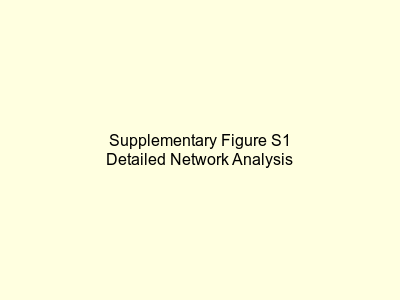
\includegraphics[width=0.8\textwidth]{supplementary/SupplementaryFigure1.png}
    \caption{Detailed build process flowchart showing the three-pass LaTeX compilation, bibliography processing, and final PDF generation stages.}
    \label{fig:supp1}
\end{figure}

\subsection{Customization Guidelines}

The template can be customized for different publication requirements by modifying the document class parameters and style definitions while maintaining compatibility with the automated build system.


\end{document}
37